\section{Problem formulation}
Using a swarm of $N$ mobile agents we want to set up a network in a mission space where the agents work as beacons in order to deliver precise positional data to entities entering the mission space.
\todo{skriv om at det er ønskelig å gjøre dette distribuert}
\subsection{Multilateration}\label[ssec]{trilat}
Multilateration is the process of determining the positions of unknown points in space by measurements of distances from known points \cite{trilat_website}. In order
to perform this task in two-dimensional space, at least three known points are needed.


Given $n\geq 3$ beacons located at positions $\mathbf{x}_{a}\in\mathbb{R}^{2},\; 0\leq a<n$ where not all points
lie on a single line the location 
of an entity, denoted by $\mathbf{y}\in\mathbb{R}^{2}$, can be determined as follows:
\begin{enumerate}
  \item The entity broadcasts signal and starts a timer at $t_{0}$.
  \item Beacons at $\mathbf{x}_{a},\; 0\leq a<n$ receive broadcasted signal and immediately responds with a packet containing $\mathbf{x}_{a}$.
  \item When receiving the packet from beacon at $\mathbf{x}_{a}$, the entity stores the time of reception in a variable $t_{1, a}$.
  \item When at least 3 beacons have responded, the entity calculates the distance
  from itself to beacon at $\mathbf{x}_{a}$: $d_{a} = \frac{1}{2}s(t_{1, a} - t_{0})$, where $s$ is the propagation speed of the signal. The factor $\frac{1}{2}$ is due to the signal traveling
  two times the distance between the entity and the beacon placed at $\mathbf{x}_{a}$ (the ping travels from the entity to the agent, and the packet
  sent by the agent travels back again).
  \item Based on the distances, $d_{a}$, and the positions of the beacons the entity can
  determine its position by calculating the point where circles centered at $\mathbf{x}_{a}$ with radii $d_{a}$ intersect.
\end{enumerate}
If sufficiently many beacons respond an ML (Maximum Likelihood) estimator of the position of the entity can be computed \cite{10.1145/381677.381693}.
Defining the error function:\begin{equation}
  e_{a}(\mathbf{y}) = s(t_{1, a} - t_{0, a}) - \norm{\mathbf{x}_{a} - \mathbf{y}} = d_{a} - \norm{\mathbf{x}_{a} - \mathbf{y}}
\end{equation}
We obtain the estimate for the position of the entity by solving:
\begin{equation}
  \mathbf{y}_{\mathrm{MMSE}} = \min_{\mathbf{y}} \mathbf{E}^{T}\mathbf{E},\quad\mathbf{E} = \begin{bmatrix}
    e_{0}(\mathbf{y})\\
    \vdots\\
    e_{n-1}(\mathbf{y})
  \end{bmatrix}
\end{equation}
The position estimation error is affected by the measurement errors, by the geometry relating sensors and target, and by the estimation algorithm \cite{trilat_error}.
As the pings sent by the entity that is to be located travel at large velocities (speed of light) the resolution of the internal clock of the entity sets a bound on the accuracy of the estimated position.
As was found in \cite{CRB_multilat}, multilateration of the unknown position of an entity is most accurate when the entity is placed nearby or within the convex hull of the beacons. Hence spreading
the beacons is desirable.
\figref{trilat_example} shows how the position of an entity can be determined from the known positions of 3 agents.
\begin{figure}[H]
  \centering
  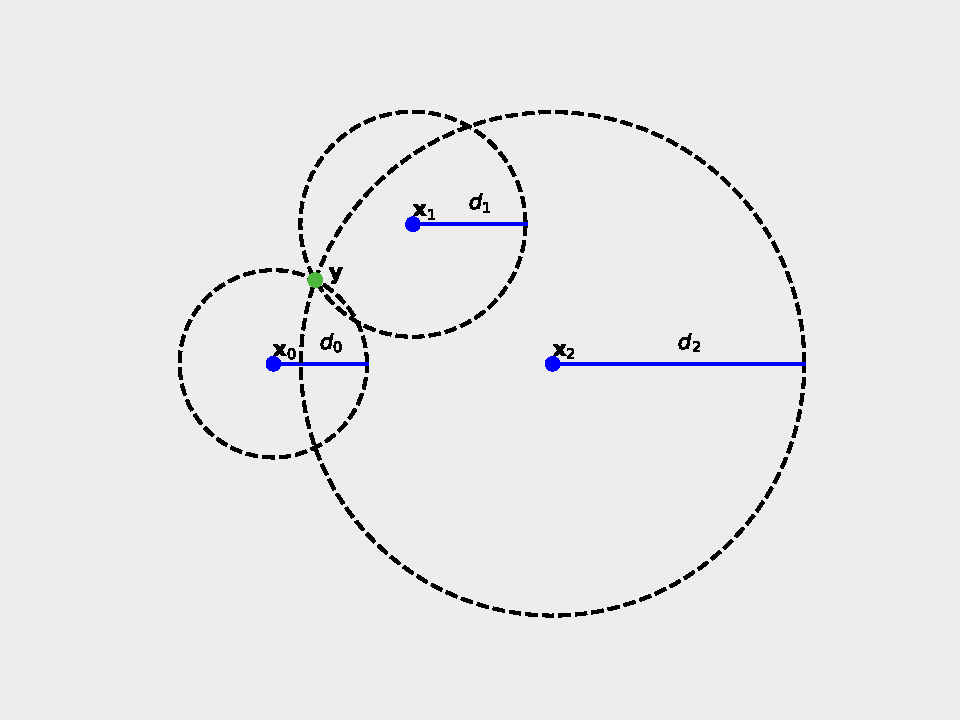
\includegraphics[width=.7\textwidth]{figs/trilateration_example.pdf}
  \caption{Position, $\mathbf{y}$, of entity determined by trilateration using known positions of $n = 3$ beacons.}
  \label[fig]{trilat_example}
\end{figure}

\subsection{Coverage}\label[secc]{coverage}
It is clear from subsection \ref{trilat} that three or more agents are needed to perform the task of multilateration. Hence a point $\mathbf{y}\in\mathcal{F}$ is said
to be \textit{covered} iff. it is within communication range of at least three agents, i.e. it is possible to determine the position of an entity placed at $\mathbf{y}$ through multilateration.

As discussed in subsection \ref{trilat} it is beneficial that agents used for multilateration spread out to some extent in order to ensure sufficient accuracy of multilateration.

\subsection{Objective function derivation}\label[secc]{obj_formulation}
The objective function presented here is inspired by \cite{sun2014escaping}, but differs in that for the purpose of multilateration, it is required that at least three agents must be within
range of a point in order for the point to be covered.

We assume we have a total of $N$ agents in a swarm $\mathcal{N}$ at our disposal. Furthermore we assume that all agents have the same maximum radius of communication:
\begin{equation}\label[eq]{homogenous_r}
  \begin{split}
    r_{a} &= r\;\forall\; a\in\mathcal{N}\\
  \end{split}
\end{equation}
Using \eqref{more_than_n_prob} we can express the probability of a point $\mathbf{y}$ being covered by the swarm as:
\begin{equation}\label[eq]{cover_prob}
  \Phi^{3^{+}}(\mathbf{X}_{\mathcal{N}}, \mathbf{y}) = 1 - \Phi^{0}(\mathbf{X}_{\mathcal{N}}, \mathbf{y}) - \Phi^{1}(\mathbf{X}_{\mathcal{N}}, \mathbf{y}) - \Phi^{2}(\mathbf{X}_{\mathcal{N}}, \mathbf{y})
\end{equation}
In order to formulate a distributed optimization algorithm, we rewrite the probability of coverage in \eqref{cover_prob} with focus on a single drone $a$.
We partition the swarm, $\mathcal{N}$, into two disjoint sets: $\{a\}$ and $\mathcal{N}\setminus\{a\}$. Using this we can rewrite \eqref{cover_prob} as:
\begin{equation}\label[eq]{distr_cover_derivation}
  \begin{split}
    \Phi^{3^{+}}(\mathbf{X}_{\mathcal{N}}, \mathbf{y}) &= 1\\
    &- \big(1-\hat{p}(\mathbf{x}_{a}, \mathbf{y})\big)\prod_{k\in\mathcal{N}\setminus\{a\}}\big(1-\hat{p}(\mathbf{x}_{k}, \mathbf{y}))\\
    &- \hat{p}(\mathbf{x}_{a}, \mathbf{y})\prod_{k\in\mathcal{N}\setminus\{a\}}\big(1-\hat{p}(\mathbf{x}_{k}, \mathbf{y}))\\
    &- \big(1-\hat{p}(\mathbf{x}_{a}, \mathbf{y})\big)\sum_{j\in\mathcal{N}\setminus\{a\}}\hat{p}(\mathbf{x}_{j}, \mathbf{y})\prod_{k\in\mathcal{N}\setminus\{a\}\setminus\{j\}}\big(1-\hat{p}(\mathbf{x}_{k}, \mathbf{y})\big)\\
    &- \hat{p}(\mathbf{x}_{a}, \mathbf{y})\sum_{j\in \mathcal{N}\setminus\{a\}}\hat{p}(\mathbf{x}_{j}, \mathbf{y})\prod_{k\in\mathcal{N}\setminus\{a\}\setminus\{j\}}\big(1-\hat{p}(\mathbf{x}_{k}, \mathbf{y})\big)\\
    &- \big(1-\hat{p}(\mathbf{x}_{a}, \mathbf{y})\big)\sum_{\mathcal{A}\in Comb(\mathcal{N}\setminus\{a\}, 2)}\prod_{j\in\mathcal{A}}\hat{p}(\mathbf{x}_{j}, \mathbf{y})\prod_{k\in\mathcal{N}\setminus\{a\}\setminus\mathcal{A}}\big(1-\hat{p}(\mathbf{x}_{k}, \mathbf{y})\big)\\
    &= 1\\
    &- \prod_{k\in\mathcal{N}\setminus\{a\}}\big(1-\hat{p}(\mathbf{x}_{k}, \mathbf{y}))\\
    &- \sum_{j\in\mathcal{N}\setminus\{a\}}\hat{p}(\mathbf{x}_{j}, \mathbf{y})\prod_{k\in\mathcal{N}\setminus\{a\}\setminus\{j\}}\big(1-\hat{p}(\mathbf{x}_{k}, \mathbf{y})\big)\\
    &- \big(1-\hat{p}(\mathbf{x}_{a}, \mathbf{y})\big)\sum_{\mathcal{A}\in Comb(\mathcal{N}\setminus\{a\}, 2)}\prod_{j\in\mathcal{A}}\hat{p}(\mathbf{x}_{j}, \mathbf{y})\prod_{k\in\mathcal{N}\setminus\{a\}\setminus\mathcal{A}}\big(1-\hat{p}(\mathbf{x}_{k}, \mathbf{y})\big)\\
  \end{split}
\end{equation}
Applying \eqref{Phi_def} to \eqref{distr_cover_derivation} yields:
\begin{equation}\label[eq]{local_coverage}
  \begin{split}
    \Phi^{3^{+}}(\mathbf{X}_{\mathcal{N}}, \mathbf{y}) &= 1 - \Phi^{0}(\mathbf{X}_{\mathcal{N}\setminus\{a\}}, \mathbf{y}) - \Phi^{1}(\mathbf{X}_{\mathcal{N}\setminus\{a\}}, \mathbf{y}) - \Phi^{2}(\mathbf{X}_{\mathcal{N}\setminus\{a\}}, \mathbf{y})\big(1-\hat{p}(\mathbf{x}_{a}, \mathbf{y})\big)\\
    &= \Phi^{3^{+}}(\mathbf{X}_{\mathcal{N}\setminus\{a\}}, \mathbf{y}) + \Phi^{2}(\mathbf{X}_{\mathcal{N}\setminus\{a\}}, \mathbf{y})\hat{p}(\mathbf{x}_{a}, \mathbf{y})\\
  \end{split}
\end{equation}
Rewriting \eqref{local_coverage} yields:
\begin{equation}
  \begin{split}
    \Phi^{3^{+}}(\mathbf{X}_{\mathcal{N}}, \mathbf{y}) &= \Phi^{3^{+}}(\mathbf{X}_{\mathcal{N}\setminus\{a\}}, \mathbf{y}) - \hat{p}(\mathbf{x}_{a}, \mathbf{y})\Phi^{3^{+}}(\mathbf{X}_{\mathcal{N}\setminus\{a\}}, \mathbf{y}) + \hat{p}(\mathbf{x}_{a}, \mathbf{y})\Phi^{2^{+}}(\mathbf{X}_{\mathcal{N}\setminus\{a\}}, \mathbf{y})\\
    &= (1-\hat{p}(\mathbf{x}_{a}, \mathbf{y}))\Phi^{3^{+}}(\mathbf{X}_{\mathcal{N}\setminus\{a\}}, \mathbf{y}) + \hat{p}(\mathbf{x}_{a}, \mathbf{y})\Phi^{2^{+}}(\mathbf{X}_{\mathcal{N}\setminus\{a\}}, \mathbf{y})\\
  \end{split}
\end{equation}
It is clear that the probability of the point $\mathbf{y}$ being covered can be seen on as an interpolation between two probability measures with the local probability of agent $a$ as the interpolation variable. Low local probability of agent $a$ means that the probability of coverage supplied the swarm as a whole depends more on the coverage supplied by
the swarm excluding agent $a$. In the extreme case where the local probability of agent $a$ is zero, the probability of covering $\mathbf{y}$ depends only on the coverage supplied by the swarm excluding agent $a$.

Higher local probability of agent $a$ means that the contribution of $a$ towards covering the point $\mathbf{y}$ is greater, thus less weight is put on the the probability of the swarm excluding agent $a$ covering the point. Instead more weight is put on the probability of at least \textit{two} other agents being able to communicate with an entity at $\mathbf{y}$. 
This is due to the fact that the probability of agent $a$ being able to communicate with said entity is higher, and we need only two or more other agents to be able to communicate with the entity at $\mathbf{y}$ to make the total number of agents covering $\mathbf{y}$ three or more.

\begin{figure}[H]
  \centering
  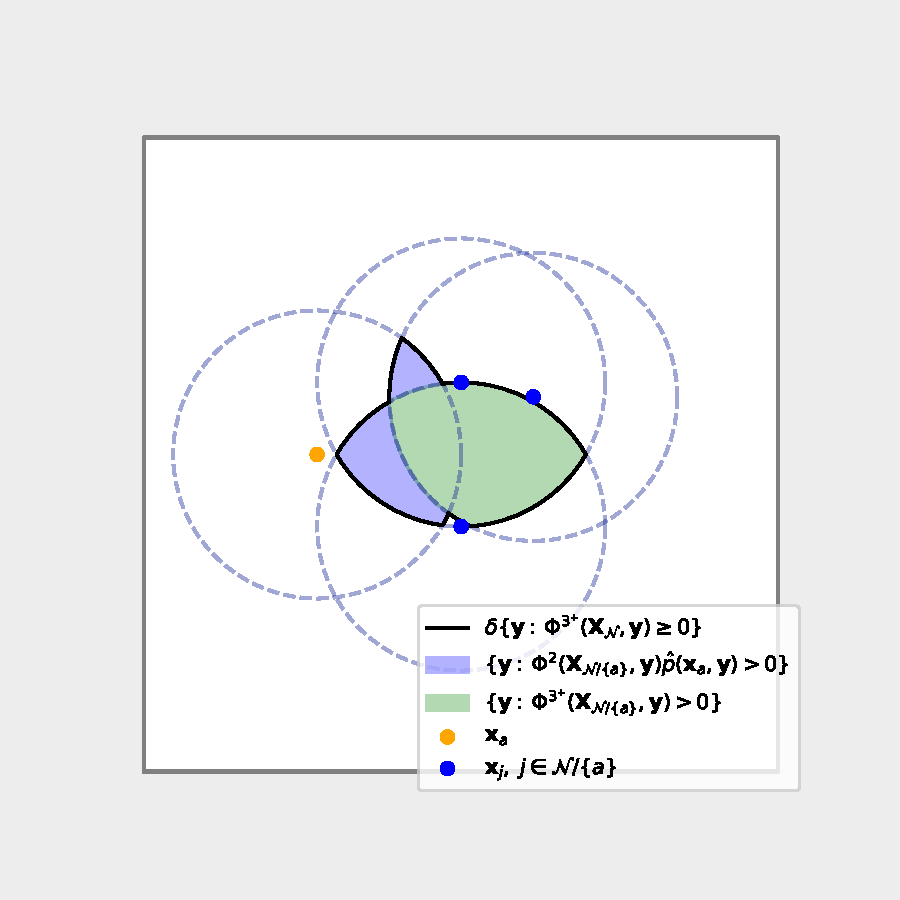
\includegraphics[width=.75\textwidth]{figs/local_objective_example.pdf}
  \caption{Non-zero regions of integrads in \eqref{rewritten_objective}. Note that perturbing the orange circle (position of agent $a$) does not affect the green region,
  as it is defined only by the intersections of the disks surrounding the blue points (other agents in the swarm).}
  \label[fig]{local_coverage_example}
\end{figure}

We note that the overall probability of coverage over the feasible space can be written as:
\begin{equation}\label[eq]{rewritten_objective}
  \begin{split}
    P(\mathbf{X}_{\mathcal{N}}) &=\int_{\mathcal{F}}\Phi^{3^{+}}(\mathbf{X}_{\mathcal{N}}, \mathbf{y})d\mathbf{y} =  \int_{\mathcal{F}}\Phi^{3^{+}}(\mathbf{X}_{\mathcal{N}\setminus\{a\}}, \mathbf{y}) + \Phi^{2}(\mathbf{X}_{\mathcal{N}\setminus\{a\}}, \mathbf{y})\hat{p}(\mathbf{x}_{a}, \mathbf{y})d\mathbf{y}\\
    &= \int_{\mathcal{F}}\Phi^{3^{+}}(\mathbf{X}_{\mathcal{N}\setminus\{a\}}, \mathbf{y})d\mathbf{y} + \int_{\mathcal{F}}\Phi^{2}(\mathbf{X}_{\mathcal{N}\setminus\{a\}}, \mathbf{y})\hat{p}(\mathbf{x}_{a}, \mathbf{y})d\mathbf{y}\\
  \end{split}
\end{equation}
We note that the first term in \eqref{rewritten_objective} is independent of the position of $a$ in both its domain and integrand. This independence is visualized in \figref{local_coverage_example}. Thus we can rewrite the overall coverage probability over $\mathcal{F}$ as:
\begin{equation}
  P(\mathbf{X}_{\mathcal{N}}) = P(\mathbf{X}_{\mathcal{N}\setminus\{a\}}) + P_{a}(\mathbf{X}_{\mathcal{N}})
\end{equation}
Where the \textit{local} probability of coverage for agent $a$ over the feasible space is defined as:
\begin{equation}\label[eq]{local_objective}
  P_{a}(\mathbf{X}_{\mathcal{N}}) = \int_{\mathcal{F}}\Phi^{2}(\mathbf{X}_{\mathcal{N}\setminus\{a\}}, \mathbf{y})\hat{p}(\mathbf{x}_{a}, \mathbf{y})d\mathbf{y}
\end{equation}

As in \cite{sun2014escaping} we note that from the viewpoint of agent $a$, the swarm can be partitioned into three disjoint sets: $\{a\}$, $\mathcal{B}_{a}$ and $\mathcal{C}_{a}$. The latter sets are defined as:
\begin{subequations}\label[eq]{B_a_and_C_a_def}
  \begin{equation}\label[eq]{neigh_def}
    \mathcal{B}_{a} = \{j\in\mathcal{N}\setminus\{a\}: \norm{\mathbf{x}_{a}-\mathbf{x}_{j}} \leq 2r\}
  \end{equation}
  \begin{equation}
    \mathcal{C}_{a} = \{j\in\mathcal{N}\setminus\{a\}: \norm{\mathbf{x}_{a}-\mathbf{x}_{j}} > 2r\}
  \end{equation}  
\end{subequations}
The set $\mathcal{B}_{a}$, from now on called the neighbours of $a$, contains all agents in the swarm, $\mathcal{N}$, whose communication disks form a non-empty intersection with that of $a$.
$\mathcal{C}_{a}$ contains all agents whose communication disks do not intersect with that of $a$.

Applying \eqref{B_a_and_C_a_def} to \eqref{local_objective} yields:
\begin{equation}
  \begin{split}
    P_{a}(\mathbf{X}_{\mathcal{N}}) &= \int_{\mathcal{F}}\Phi^{2}(\mathbf{X}_{\mathcal{N}\setminus\{a\}}, \mathbf{y})\hat{p}(\mathbf{x}_{a}, \mathbf{y})d\mathbf{y}\\
    &= \int_{\mathcal{F}}\Big(\Phi^{2}(\mathbf{X}_{\mathcal{B}_{a}}, \mathbf{y}) + \Phi^{2}(\mathbf{X}_{\mathcal{C}_{a}}, \mathbf{y}) + \Phi^{1}(\mathbf{X}_{\mathcal{B}_{a}}, \mathbf{y})\Phi^{1}(\mathbf{X}_{\mathcal{C}_{a}}, \mathbf{y})\Big)\hat{p}(\mathbf{x}_{a}, \mathbf{y})d\mathbf{y}
  \end{split}
\end{equation}
Partitioning the domain of integration into the visible set and invisible set of agent $a$, and noting that $\hat{p}(\mathbf{x}_{j}, \mathbf{y}) = 0\;\forall\;j\in\mathcal{C}_{a},\;\mathbf{y}\in V_{a}$ such that
$\Phi^{n}(\mathbf{X}_{\mathcal{C}_{a}}, \mathbf{y}) = 0\;\forall\;n\in\mathbb{Z}^{+},\;\mathbf{y}\in V_{a}$, and $\hat{p}(\mathbf{x}_{a}, \mathbf{y}) = 0\;\forall\;\mathbf{y}\in U_{a}$ yields:
\begin{equation}\label[eq]{local_objective_derivated}
  \begin{split}
    P_{a}(\mathbf{X}_{\mathcal{N}}) &= \int_{V_{a}}\Big(\Phi^{2}(\mathbf{X}_{\mathcal{B}_{a}}, \mathbf{y}) + \Phi^{2}(\mathbf{X}_{\mathcal{C}_{a}}, \mathbf{y}) + \Phi^{1}(\mathbf{X}_{\mathcal{B}_{a}}, \mathbf{y})\Phi^{1}(\mathbf{X}_{\mathcal{C}_{a}}, \mathbf{y})\Big)\hat{p}(\mathbf{x}_{a}, \mathbf{y})d\mathbf{y}\\
    &+ \int_{U_{a}}\Big(\Phi^{2}(\mathbf{X}_{\mathcal{B}_{a}}, \mathbf{y}) + \Phi^{2}(\mathbf{X}_{\mathcal{C}_{a}}, \mathbf{y}) + \Phi^{1}(\mathbf{X}_{\mathcal{B}_{a}}, \mathbf{y})\Phi^{1}(\mathbf{X}_{\mathcal{C}_{a}}, \mathbf{y})\Big)\hat{p}(\mathbf{x}_{a}, \mathbf{y})d\mathbf{y}\\
    &= \int_{V_{a}}\Phi^{2}(\mathbf{X}_{\mathcal{B}_{a}}, \mathbf{y})p(\norm{\mathbf{x}_{a}-\mathbf{y}})d\mathbf{y} = L(\mathbf{X}_{\mathcal{B}_{a}\cup\{a\}})
  \end{split}
\end{equation}
Thus the local probability of coverage for an agent $a$ is dependent on the position, $\mathbf{x}_{a}$, of agent $a$ in both domain and integrand, and the positions of the neighbours of agent $a$.
We call the swarm consisting of $a$ and its neighbours agent $a$'s local swarm.\clearpage

In order to encourage spread of agents in situations where small perturbations of the position of an agent
causes no or minor changes to the local probability of coverage, we introduce a term causing an agent $a$ to move away
from another agent $j$. When agents are close to each other we want this term to induce some velocity in the agents causing
them to spread. Furthermore we want this velocity to decrease with increasing spread. Due to this we model the proximity of two agents as:
\begin{equation}\label[eq]{proximity_func}
  D(\mathbf{x}_{a}, \mathbf{x}_{j}) = k_{1}e^{-k_{2}\norm{\mathbf{x}_{a} - \mathbf{x}_{j}}}
\end{equation}
The function has two tunable parameters, $k_{1}$ and $k_{2}$, whose effects are show in \figref{cdr}.

Using \eqref{local_objective_derivated} and \eqref{proximity_func}  We now state the \textit{local} objective for an agent $a$ as:
\begin{equation}\label[eq]{local_objective_func}
  H(\mathbf{X}_{\mathcal{B}_{a}\cup\{a\}})  = L(\mathbf{X}_{\mathcal{B}_{a}\cup\{a\}})  - \sum_{j\in\mathcal{B}_{a}}D(\mathbf{x}_{a}, \mathbf{x}_{j})
\end{equation}
Due to the negative sign in front of the sum of proximity functions, we will refer to this as the active dispersion term.
\begin{figure}[H]
  \centering
  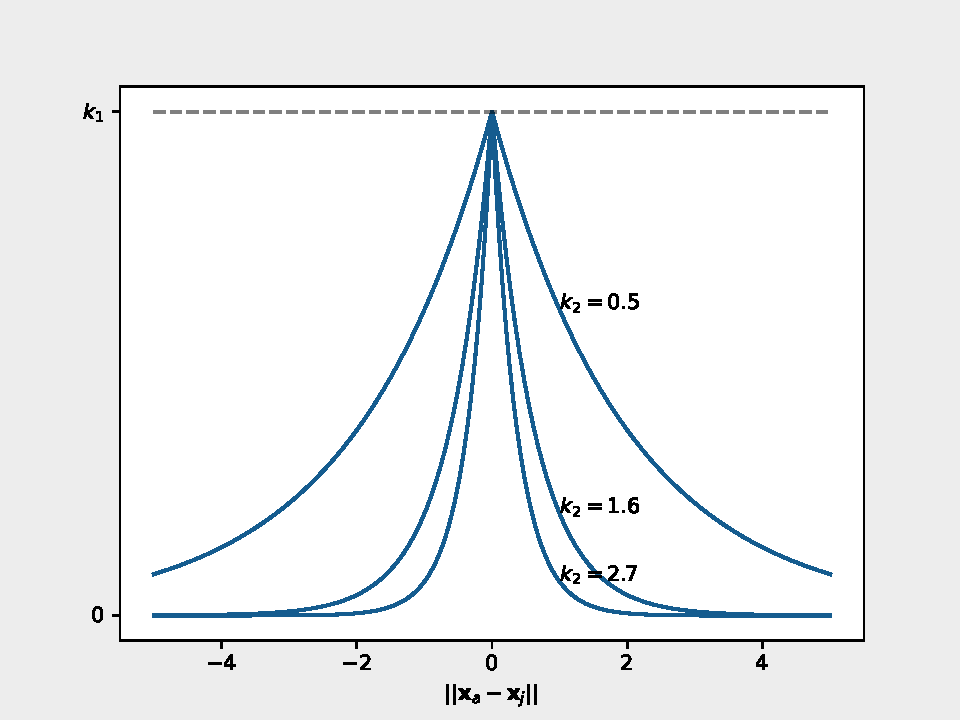
\includegraphics[width=.7\textwidth]{figs/close_dist_repell_example.pdf}
  \caption{Proximity term in \eqref{proximity_func} for an agent, $a$, and its neighbour, $j$.}
  \label[fig]{cdr}
\end{figure}

\subsection{Constraints}\label[secc]{constraints}
It is clear from subsection \ref{trilat} that agents used as beacons in a multilateration scheme cannot be positioned on a straight line, as this would make it impossible
to uniquely determine the unknown position of an entity. Due to the fact that only agents close to the entity whose position is to be determined will
take part in the multilateration scheme, we impose only that agents that together can be used for multulateration must satisfy the non-linear position requirement.

For an agent $a$ with $N$ neighbours $j\in\mathcal{B}_{a},\:|B_{a}|=N$ we construct a matrix $\mathbf{V}$ according to:
\begin{equation}\label[eq]{V_def}
  \mathbf{V}(\mathbf{X}_{\mathcal{B}_{a}}) = \begin{bmatrix}
    \mathbf{X}_{\mathcal{B}_{a, 0}}-\mathbf{X}_{\mathcal{B}_{a, 1}}&\hdots&\mathbf{X}_{\mathcal{B}_{a, 0}}-\mathbf{X}_{\mathcal{B}_{a, N-1}}.
  \end{bmatrix}
\end{equation}
If agent $a$ has less than two neighbours, or all of agent $a$'s neighbours are positioned on a straight line, the matrix $\mathbf{V}(\mathbf{X}_{\mathcal{B}_{a}})$ will not span $\mathbb{R}^{2}$, i.e. $\mathrm{Rank}(\mathbf{V}(\mathbf{X}_{\mathcal{B}_{a}})) < 2$ \todo{citation for matrix rank}.

Assuming that agent a has two or more agents, $|\mathcal{B}_{a}|\geq 2$, and that all neighbours of $a$ are positioned on a straight line. It is then desirable that agent $a$ is positioned sufficiently far away from the line. This constraint is implemented as follows:
Wihout loss of generality we define:
\begin{subequations}\label[eq]{vl}
  \begin{align}
    \mathbf{v}(\mathbf{x}_{a}) &= \mathbf{x}_{a} - \mathbf{X}_{\mathcal{B}_{a}, 0}\\
    \mathbf{l} &= \mathbf{X}_{\mathcal{B}_{a}, 1} - \mathbf{X}_{\mathcal{B}_{a}, 0},
  \end{align}
\end{subequations}
meaning $\mathbf{v}(\mathbf{x}_{a})$ is the vector from agent $a$ to its first neighbour, and $\mathbf{l}$ is the vector between agent $a$'s first and second neighbour. Thus $\mathbf{l}$ is paralell to the line 
that goes through all of agent $a$'s neighbours.
Using (3.98) in \cite{projection} to project $\mathbf{v}(\mathbf{x}_{a})$ into $\mathbf{l}$ we get the component of $\mathbf{v}(\mathbf{x}_{a})$ that is parallel to the line
through agent $a$'s neighbour $i$ and $j$:
\begin{equation}
  \mathbf{v}_{\parallel}(\mathbf{x}_{a}) = \frac{\mathbf{v}(\mathbf{x}_{a})^{T}\mathbf{l}}{\mathbf{l}^{T}\mathbf{l}}\mathbf{l}
\end{equation}
The component of $\mathbf{v}(\mathbf{x}_{a})$ perpendicular to the line through agent $a$'s
neighbours is obtained as:
\begin{equation}
  \mathbf{v}_{\perp}(\mathbf{x}_{a}) = \mathbf{v}(\mathbf{x}_{a}) - \mathbf{v}_{\parallel}(\mathbf{x}_{a})
\end{equation}
Now the distance from agent $a$ to the line through its neighbours can be computed as:
\begin{equation}
  \norm{\mathbf{v}_{\perp}(\mathbf{x}_{a})} = \norm{\mathbf{v}(\mathbf{x}_{a}) - \frac{\mathbf{v}(\mathbf{x}_{a})^{T}\mathbf{l}}{\mathbf{l}^{T}\mathbf{l}}\mathbf{l}}
\end{equation}
Seen as it is impossible to place and agent such that it lays on a straight line through all it's neighbours if the neigbhours do not already
lay on a straight line we demand that the non-linear position constraint be fulfilled only when $\mathrm{Rank}(\mathbf{V}(\mathbf{X}_{\mathcal{B}_{a})}) < 2$, where $\mathbf{V}(\cdot)$ is defined in \eqref{V_def}. The non-linear position constraint is defined as:
\begin{equation}\label[eq]{non_lin_pos}
    \norm{\mathbf{v}(\mathbf{x}_{a}) - \frac{\mathbf{v}(\mathbf{x}_{a})^{T}\mathbf{l}}{\mathbf{l}^{T}\mathbf{l}}\mathbf{l}}\geq d_{min} 
\end{equation}
where $d_{min}$ is a tunable parameter that defines how close an agent is allowed get to the line through it's neigbhours, and $\mathbf{v}$ and $\mathbf{l}$
are defined in \eqref{vl}.

We also impose that any two agents must be some minimum distance apart at any given time. This is due to the fact that agents colliding could cause damage to the hardware, and possibly render them unusable.
This constraint is modelled as:
\begin{equation}
  \norm{\mathbf{x}_{a} - \mathbf{x}_{j}} \geq r_{min} \;\forall\;j\in\mathcal{B}_{a},
\end{equation}
where $r_{min}$ is a tunable parameter that sets a limit to how close an agent can be positioned to any of its neihbours.\clearpage
\subsection{Optimization problem formulation}
The non-linear position constraint \eqref{non_lin_pos} presented in \ref{constraints} is dependent on the neighbour set of agent $a$, $\mathcal{B}_{a}$, as it should only be imposed if the 
neigbours of agent $a$ lay on a straight line. Using the objective function in \eqref{local_objective_func} and the constraints in discussed in \ref{constraints} we define the optimization problem:
\begin{subequations}\label[eq]{local_opt_prob}
  \begin{align}
    \begin{split}\label[eq]{totally_objective}
      &\max_{\mathbf{x}_{a}}\;H(\mathbf{X}_{\mathcal{B}_{a}\cup\{a\}})\\
    \end{split}\\
    \mathrm{s.t.}\;
    \begin{split}
      &\mathbf{x}_{a}\in\mathcal{F}
    \end{split}\\
    \begin{split}\label[eq]{min_two_neig}
      &|\{j\in\mathcal{B}_{a}: \norm{\mathbf{x}_{a} - \mathbf{x}_{j}} \leq 2r\}|\geq 2
    \end{split}\\
    \begin{split}
      &\norm{\mathbf{x}_{a} - \mathbf{x}_{j}} \geq r_{min}\;\forall\;j\in\mathcal{B}_{a}
    \end{split}\\
    \begin{split}\label[eq]{non_linear_neighb}
      &\norm{\mathbf{v}(\mathbf{x}_{a}) - \frac{\mathbf{v}(\mathbf{x}_{a})^{T}\mathbf{l}}{\mathbf{l}^{T}\mathbf{l}}\mathbf{l}}\geq d_{min},\quad\mathrm{iff.}\;\mathrm{Rank}(\mathbf{V}(\mathbf{X}_{\mathcal{B}_{a}}))<2
    \end{split}
\end{align}
\end{subequations}
where $\mathbf{V}(\cdot)$ is defined in \eqref{V_def} and $\mathbf{v}(\cdot)$ and $\mathbf{l}$ are defined in \eqref{vl}.

In situations where $\frac{\partial L(\mathbf{X}_{\mathcal{B}_{a}\cup\{a\}})}{\partial \mathbf{x}_{a}} = 0$ the solution of \eqref{totally_objective} will be achieved at the position $\mathbf{x}_{a}$ that minimizes the dispersion term in \eqref{local_objective_func}.
This will cause agent $a$ to move as far away from its neighbours as possible. Such behaviour is undesirable as this might render agent $a$ neighbour-less. For an agent 
$a$ without neighbous we have $\mathcal{B}_{a} = \emptyset$ and hence $H(\mathbf{X}_{\mathcal{B}_{a}\cup\{a\}}) \equiv 0$. Thus re-optimization will result in $\mathbf{x}_{a}$ being unaltered, causing agent $a$
to stay at $\mathbf{x}_{a}$ indefinately. To prevent such behaviour we impose the constraint \eqref{min_two_neig}. This will prevent agent $a$ from completely disconnecting from its local swarm. 

Furthermore we observe that Rank$(\mathbf{V}(\mathbf{X}_{\mathcal{B}_{a}}))<2$ if either all neigbhours of agent $a$ lie on a straight line or agent $a$ has less than two neighbours. If agent $a$ has less than
two neighbours it is not possible to draw a line between the neighbours of agent $a$, and thus the non-linear neighbour constraint \eqref{non_linear_neighb} is undefined. This further motivates imposing the constraint that
agent $a$ should have at least two neighbours at the solution to \eqref{local_opt_prob}.

The optimization problem formulated in \eqref{local_opt_prob} is non-convex \cite{NoceWrig06_convex_prob}. The objective function is generally non-concave and the constraints form a non-convex feasible set. In 
\figref{objective_example} a visualization of the objective function is shown for an agent with 5 neighbours.
\begin{figure}[H]
  \centering
  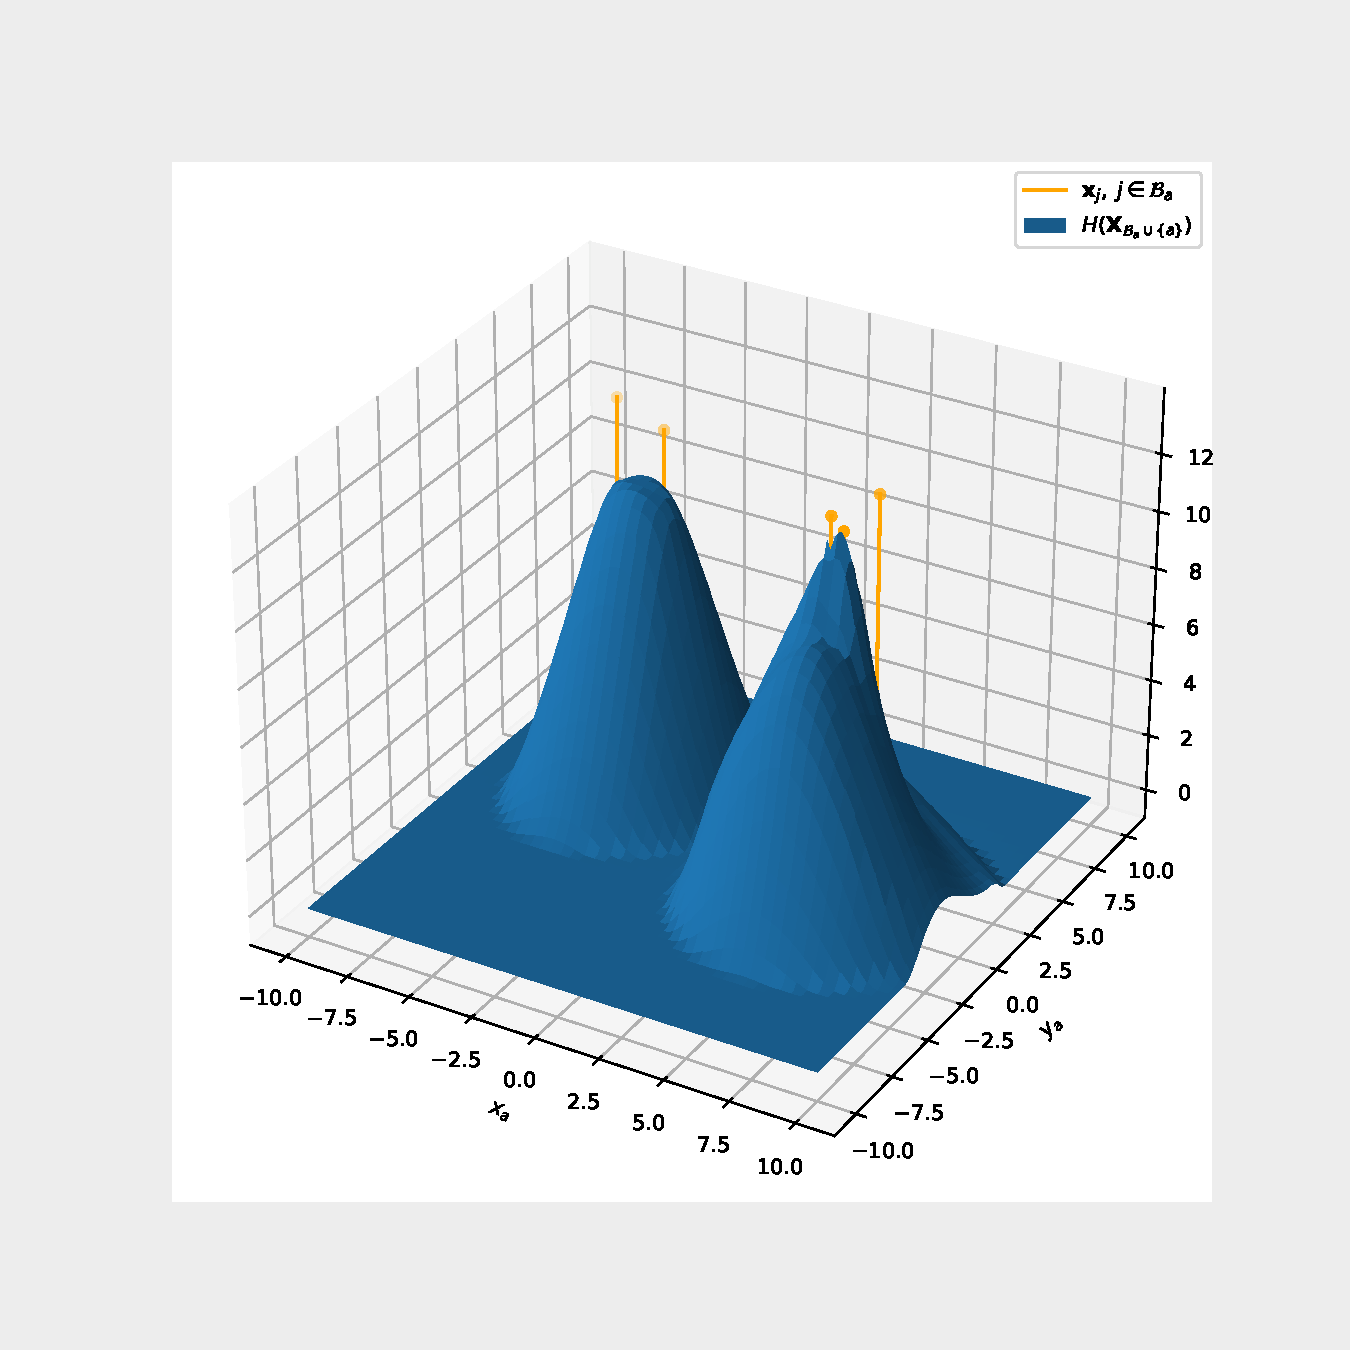
\includegraphics[width = .8\textwidth]{figs/objective_example.pdf}
  \caption{Objective function in \eqref{totally_objective} for agent $a$ with $|B_{a}| = 5$.}
  \label[fig]{objective_example}
\end{figure}